\section{Experiment 1: Analyzing Performance of TCP Variants}

This experiment analyzed the performance of different TCP variants over a setup consisting of a single TCP stream and a single CBR flow. The performance of the TCP variants were analyzed over a range of different packet sizes and transmission rates assigned to the CBR. We analyze the results of this experiment in two parts. First, by looking at the performance of the variants over an increasing range of CBR packet sizes, while the rate of the CBR is constant at 2Mbps. Second, we look at the performance of the variants over an increasing range of CBR flows - from 1 Mbps to 10 Mbps, while the size of the packet is held constant at 3,000 bytes.

When holding the CBR steady, at 2Mbps, none of the variants experienced any packet loss over the range of increasing packet sizes, from 500 bytes to 8,000 bytes. The average and end-to-end latency as well as the throughput for TCPs , Reno, NewReno and Tahoe were all the same. The throughput hovered around 1 Mbps as the size of packets increased and the average latency hovered around .02 seconds. The average and end-to-end latency of TCP Vegas was slightly smaller, likely because Vegas never saturates the full capacity of the link. Doing so, would imply congestion and the throughput would decrease. The throughput for Vegas hovered at just under .99 Mbps as the size of the packets increased and the latency hovered around .005 seconds.

\begin{figure}[!htbp]
	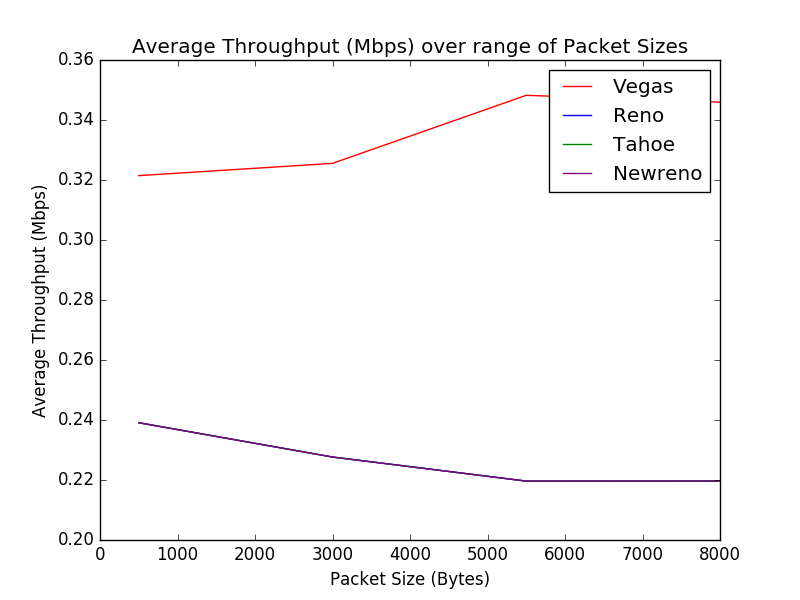
\includegraphics[scale=0.4]{P1.png}
	\caption{This figure plots the average throughput of each TCP variant over a range of CBR flow rates. The packet size is initialized to 3,000 bytes.}
	\label{a:label}
\end{figure}

When the packet size is held steady, at 3,000 bytes and the CBR flow is increased from 1 Mbps to 10 Mbps, all four variants suffer packet loss. Reflected in Figure 3, TCPs Reno, NewReno and Tahoe suffer their first packet drops at a CBR of 7 Mbps. TCP Vegas does not suffer any packet drops, but the throughput in consistently lower than the other variants, as it is reducing its congestion window size to reflect the increasing RTT of the packets. TCP Vegas takes preventative measures to avoid packet loss. The other variants make changes only in the aftermath of packet loss. To prevent congestion, Vegas records the round trip time (RTT) of packets and adjusts its congestion window according to any delay.  Vegas does not experience packet loss until the CBR rate is 9Mbps.

\begin{figure}[!htbp]
	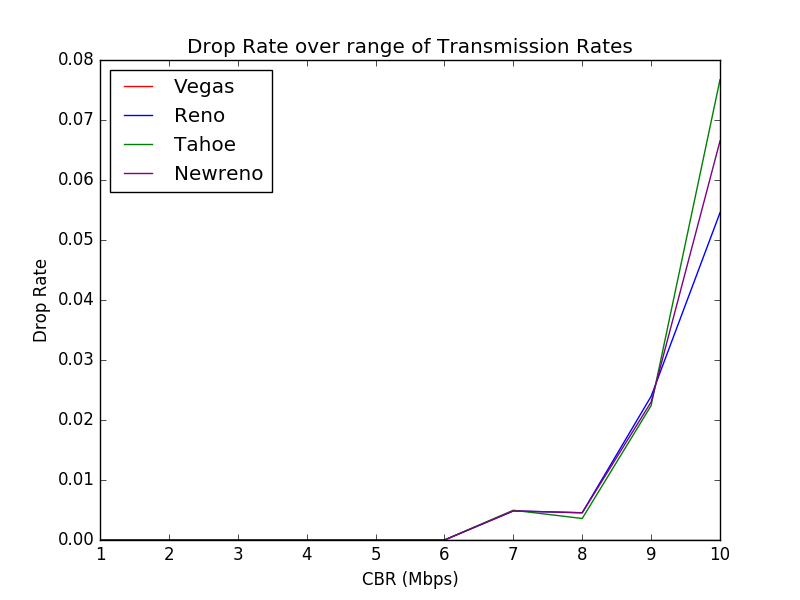
\includegraphics[scale=0.4]{P2.png}
	\caption{This figure plots the number of packets dropped by each TCP variant over a range of CBR flow rates. The packet size is initialized to 3,000 bytes.}
	\label{a:label}
\end{figure}

Each variant is consistent, only in that they wait until receiving 3 duplicate-acknowledgements or retransmit timeouts before retransmitting the first lost packet. 

Given low-to-moderate levels of congestion, TCP Vegas is able to efficiently decrease its congestion window size, before experiencing packet loss, and thus is able to maintain 0 packet loss while its counterparts are unable to. However, once some threshold is reached, Vegas will suffer packet loss and will no longer the most efficient variant in terms of dealing with multiple packet losses. NewReno, handles multiple packet losses better than its counterparts. After the first packet loss is identified by a triple duplicate acknowledgement, or by a retransmission timeout, NewReno assumes that any packet following a partial acknowledgment is lost. This makes the retransmission of packets much faster and accounts for the increase in throughput experienced by NewReno in Figure 2.


